\chapter{BASIC GROUP THEORY}

\section{Basic Definitions and Simple Example}
\textbf{Definition 1.1, Group} A set $\{G: a, b, c\dots\}$ is sai to form a group if there is an operaton called \textit{group multiplication}, which associates any given pair of elements $a, b \in G$ with a well-defined product $a \cdot b$ which is also an element of $G$, such that the following  condition are satisfied:
\begin{itemize}
  \item The operation $\cdot$ is associative, $a \cdot \left(b \cdot c\right) = \left(a\cdot b \right) \cdot c$for all $a, b, c \in G$;
  \item Among the elements of $G$, there is an element $e$, called the identity;
  \item For each $a \in G$, there is an inverse element, $a \cdot a^{-1}=e$.
\end{itemize}

\textrm{Example 1}: The $C_{2}$ group.
There are two group elements with the multiplication table in Tab.~\ref{tab:1-1}
\begin{table}
  \centering
  \begin{tabular}{c c}
    \hline
    e & a \\
    a & e \\
    \hline
  \end{tabular}
  \caption{Group Multiplication Table of $C_{2}$}
  \label{tab:1-1}
\end{table}
In physics, the spatial inversion transformation and identity form such a group.

\textit{Example 3}: There is one and only one three-element group called $C_{3}$ and the multiplication table is Tab.~\ref{tab:1-2}.
\begin{table}
  \centering
  \begin{tabular}{c c c}
    \hline \\
    e & a & b \\
    a & b & e \\
    b & e & a \\
    \hline
  \end{tabular}
  \caption{Group Multiplication Table of $C_3$}
  \label{tab:1-2}
\end{table}
Since $ab=e$ we conclude $b=a^{-1}$, we can denote the three elements by $\{e, a, a^{-1}\}$ with the requirement $a^{3}=e$.
Concrete examples of the the group $C_{3}$ are: the numbers $\left( 1, e^{i2\pi/3}, e^{-i2\pi/3}\right)$ with the usual rules of multiplication; the symmetry operations of the equilater trangle in the plane.

All these groups mentioned are examples of \textit{cyclic} group $C_{n}$ which have the general structure $\{e, a, a^{2}, \dots, a^{n-1}; a^{n}=e\}$ where $n$ can be any positive integer.

\textbf{Definition 1.2, Abelian group} An \textit{abelian group} $G$ is none for which the group multiplication is commutative.

\textbf{Definition 1.3, Order} The \textit{order} of a group is the number of elements of the group.

The cyclic groups $C_{n}$ described abover are all abelian.
Most interesting groups are not abelian.

\textrm{Example 4}: The simplist non-cyclic group is of order $4$.
It is usually called the \textit{dihedral group} denoted by $D_{2}$ with the multiplication table Tab.~\ref{tab:1-3}
\begin{table}
  \centering
  \begin{tabular}{c c c c}
    \hline
    e & a & b & c \\
    a & e & c & b \\
    b & c & e & a \\
    c & b & a & e \\
    \hline
  \end{tabular}
  \caption{Group Multiplication Table of $D_2$}
  \label{tab:1-3}
\end{table}

A visualize of this abelian group is by its association to a geometrical symmetry by considering the configuration of
Fig.~\ref{fig:1-1}.
\begin{figure}[h]
  \centering
  \begin{tikzpicture}
    \draw (0,0) -- (0,2) -- (4,2) -- (4,0) -- (0,0);
    \draw (0,1) -- (4,1);
    \draw (2,0) -- (2,2);
    \node [left] at (0,1) {$4$};
    \node [right] at (4,1) {$2$};
    \node [below] at (2,0) {$3$};
    \node [above] at (2,2) {$1$};
  \end{tikzpicture}
  \caption{A configuration with $D_2$ symmetry.}
  \label{fig:1-1}
\end{figure}
Applying the following tansformations on this figure: (i) leaving the figure unchanged; (ii) reflection about the vertical axis $(1,3)$; (iii) reflection about the horizontal axis $(2,4)$; and (iv) rotation of the figure in the plane around the center by $\pi$.
It is straightforward to check that the multiplication thable obtained through these geomentric constructions reproduces Tab.~\ref{tab:1-3}.

\section{Further Examples, Subgroups}
The smallest \textit{non-abelian group} is of order $6$.
It can be generated from the symmetry transformations of the geometric configuration of Fig.~\ref{fig:1-2}.
\begin{figure}[b]
  \centering
  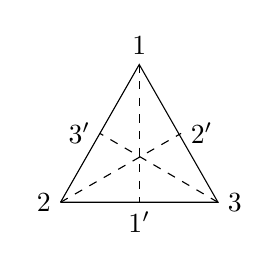
\begin{tikzpicture}
    \draw (0,0) -- (2,0) -- (1, 1.75) -- (0,0);
    \draw [dashed] (0,0) -- (1.531,0.875);
    \draw [dashed] (2,0) -- (0.5,0.875);
    \draw [dashed] (1,1.75) -- (1,0);
    \node [above] at (1,1.75) {$1$};
    \node [right] at (2,0) {$3$};
    \node [left] at (0,0) {$2$};
    \node [below] at (1,0) {$1'$};
    \node [right] at (1.531,0.875) {$2'$};
    \node [left] at (0.5,0.875) {$3'$};
  \end{tikzpicture}
  \caption{A configuration with $D_3$ symmetry}
  \label{fig:1-2}
\end{figure}
The operations are (1) the identity transformation, (ii) reflections about the axes $\left(1,1'\right)$ and so on and (iii) the rotations about the center by angles $\frac{2\pi}{3}$ and $\frac{4\pi}{3}$.
They form the \textit{dihedral group} $D_{3}$.
The reflecvtions interchange two fo the labels, leaving the remaining one unchanged, which we denote the oberation by $\left( 12\right)$.
For rotation counter-clockwise by $\frac{2\pi}{3}$ and $\frac{4\pi}{3}$ we deonte by $\left(321\right)$ and $\left(123\right)$ respectively.
One can see that there is a one-to-one correspondence between these symmetry transformations and the permutations of ther tree label whic form the permutation group $S_{3}$ in next section.
The group multiplication table is shown in Tab.~\ref{tab:1-4}.
\begin{table}
  \centering
  \begin{tabular}{c c c c c c}
    \hline \\
    $e$ & $\left(12\right)$ & $\left(23\right)$ & $\left(31\right)$ & $\left(123\right)$ & $\left(321\right)$ \\
    $\left(12\right)$ & $e$ & $\left(123\right)$ & $\left(321\right)$ & $\left(23\right)$ & $\left(31\right)$ \\
    $\left(23\right)$ & $\left(321\right)$ & $e$ & $\left(123\right)$ & $\left(23\right)$ & $\left(12\right)$ \\
    $\left(31\right)$ & $\left(123\right)$ & $\left(321\right)$ & $e$ & $\left(12\right)$ & $\left(23\right)$ \\
    $\left(123\right)$ & $\left(31\right)$ & $\left(12\right)$ & $\left(23\right)$ & $\left(321\right)$ & $e$ \\
    $\left(321\right)$ & $\left(23\right)$ & $\left(31\right)$ & $\left(12\right)$ & $e$ & $\left(123\right)$ \\
    \hline
  \end{tabular}
  \caption{Group Multiplication Table of $D_3$ or $S_3$}
  \label{tab:1-4}
\end{table}

\textbf{Definition 1.4, Subgroup} A subset $H$ of a group $G$ which forms a group under the same multiplication law as $G$ is said to form a \textit{subgroup} of $G$.

\textrm{Example 1} The group $S_{3}$ has four distinct subgroups consisting of the elements $\{e, \left(12\right)\}, \{e, \left(23\right)\}, \{e, \left(31\right)\}$ and $\{e, \left(123\right), \left(321\right)\}$ respectively.
The first three subgroups are identcal to the $C_{2}$ group.
The last one has the structure of $C_{3}$.
This can be seen by refering to the geometrical transformations in Fig.~\ref{fig:1-2}.

In many applications, the group elements carry labels which are continuous parameters.
These are \textit{continuous groups}.
Group of rotations in Euclidean spaces, and groups of continuous translations areprominent examples.
For later useage, we refere to the groups of ratiotions in space as $R\left(n\right)$ and the comined groups of rotations and translations in the same space as $E_{n}$.
The latter two are examples of \textit{Euclidean groups}.

Any set of invertible $n\times n$ matrices, which includes the unit matrix and which is closed under matrix multiplication, forms a \textit{matrix group}.
Important examples are:
\begin{itemize}
  \item the general \textit{linear group} $GL \left(n\right)$ consisting of all invertible $n\times n$ matrices;
  \item the \textit{unitary group} $U \left(n\right)$ consiting of unitary matrices, $U U^{\dagger} =1$;
  \item the \textit{special unitary group} $SU\left(n\right)$ consisting of unitary matrices with \textit{unit determinant} $\det{U}=1$;
  \item the \textit{orthogonal group} $O \left(n\right)$ consisting of real orthogonal matrics $OO^{T} = 1$.
\end{itemize}

These are examples of classical groups which occupy a central placew in group representation theory and have many applications in various branches of mathematics and physics.
Clearly, $SU\left(n\right)$ and $O\left(n\right)$ are subgroups of $U\left(n\right)$ which, in turn, is a subgroup of $GL\left(n\right)$.

\section{The Rearrangement Lemma and the Symmetric Group}
\textbf{Rearrangement Lemma:} If $p, b, c \in G$ and $pb = pc$ then $b=c$.

This result means: if $b$ and $c$ are distinct elements of $G$, then $pb$ and $pc$ are also distinct.
Therefore, if all the elements of $G$ are arranged in a sequencse and are multiplied on the left (right) by a given element $p$, the resulting squence is just a rearrangement of the original one.

Let us consider a finite group of order $n$, which is $\{g_{i}; i = 1,\dots, n\}$.
Multiply by $h\in G$ which is $g_{h_{i}} = hg_{i}$, then these $h_{i}$ are just the rearrangement of the label $i = 1, \dots, n$ and they must be distinct with each other due to the rearrangement lemma.

We introduce the \textit{group of permutations}.
An arbitrar permutation of $n$ objects wiht be denoted by
\begin{equation*}
  p =
  \begin{pmatrix}
    1 & 2 & 3 & \dots & n \\
    p_{1} & p_{2} & p_{3} & \dots & p_{n}
  \end{pmatrix}
\end{equation*}
The set of $n!$ permutations of $n$ objects form a group $S_{n}$ called the \textit{permutations group} or the \textit{symmetric group}.

A more compact and convenient notation for permution s is based on the \textit{cycle structure} which can be explained by example.
\begin{equation*}
  p =
  \begin{pmatrix}
    1 & 2 & 3 & 4 & 5 & 6 \\
    3 & 5 & 4 & 1 & 2 & 6
  \end{pmatrix}
\end{equation*}
We have the following replacement $1 \to 3 \to 4 \to 1$.
These three objects form a \textit{three-cycle} to tbe denoted by $\left(134\right)$.
Similarly, we have $\left(25\right)$ and $\left(6\right)$.
Then the \textit{cycle notation} $\left(134\right) \left(25\right) \left(6\right)$ uniquely specifies the permutation.
In this notation, the identity element consists of $n$ one-cycles,and inverse element is simply the same numbers in reverse order, i.e. $\left(p_{1}, p_{2}, \dots, p_{m} \right)^{-1} = \left(p_{m}, \dots, p_{2}, p_{1}\right)$.
We have already use this notation in Tab.~\ref{tab:1-4}.

\textbf{Definition 1.5, Isomorphism}: Two groups $G$ and $G'$ are said to be \textit{isomorphic} if there exists a one-to-one correspondence between their elements with preserves the law of group multiplication.
In other words, if $g_{i} \in G \leftrightarrow g_{i}' \in G'$ and $g_{1}g_{2} = g_{3}$ in $G$, gives $g_{1}'g_{2}'= g_{3}'$ in $G'$ and vice versa.

\textrm{Exampels}: (i) The group consisting of the numbers $\{\pm 1, \pm i \}$ with respect to the usual multiplication is isomorphic to the cyclic group $C_{4} = \{1, i, i^{2}=-1, i^{3} = -i; i^{4} = 1\}$.
(ii) The dihedral group $D_{3}$ is isomorphic to the symmetryc group $S_{3}$ defined above.

\textbf{Theorem 1.1, Cayley}: Every group $G$ of order $n$ is isomorphic to a subgroup of $S_{n}$.

\textrm{Example 1}: The cyclic group of order $3$, $\{C_{3}: e, a, b=a^{2}\}$ is isomorphic to the subgroup of $S_{3}$ consisting of the elements $\{e, \left(123\right), \left(321\right)\}$.

\textrm{Example 2}: The dihedral group $\{ D_{2}: e, a, b, c\}$ in Tab.~\ref{tab:1-3} is somorphic to the subgroup of $S_{4}$ consisting of the elements $\{ e, \left(12\right)\left(34\right), \left(13\right)\left(24\right), \left(14\right)\left(23\right)\}$.

An interesting general feature due to the Rearrangement Lemma is that no element other than the identity in a subgroup of $S_{n}$ which is isomorphic to a group of order $n$ in the specified way can contain one-cycles\footnote{The presence of a one-cycle means that a particular group element is uchanged upon left multiplication by another element which is not the identity. This contradicts the Rearrangement Lemma: $ba = a = e a$ then $b=e$.}
Furthermore, the cycles which do occur in any permutation associated with a given group element must alll be of the same length\footnote{If $g\in G$, have two cycle with differenct length $l_{1} < l_{2}$, then $g^{l_{1}}\in G$ contain one-cycle.}.
An interesting consequence of this result is that: if the order $n$ of a group is a prime number, then the corrsponding subgroup of $S_{n}$ can only contain unfactorized full $n-$fycles.
These correspond to elements of the cyclic group of order $n$.

\textbf{Theorem 1.2}: If the order $n$ of a group is a prime number, it must be isomorphic to $C_{n}$.

\section{Classes and Invariant Subgroups}
The elements of a group $G$ can be partitioned into conjugate classes and cosets.

\textbf{Definition 1.6} (Conjugate Elements): An element $b\in G$ is said to be \textit{conjugate} to $a \in G$ if there exists another group $p \in G$ such that $ b = p a p^{-1}$. We shal denote the conjugation relation by the symbol $\sim$.

Conjugation is an \textit{equivalence relation}: (i) each element is conjugate to itself $a \sim a$ (reflexive); (ii) if $a \sim b$ then $b \sim a$ (symmetric); and (iii) if $a \sim b$ and $b \sim c$, then $a \sim c$ (transitive).
It is well known that any equivalence relation provides a unique way to classify the elements of set.

\textbf{Definition 1.7} (Conjugate Class): Elements of a group which are conjugate to each other are said to form a (conjugate) class.

Each element of a group belongs to one and only one class.
The identity element forms a class all by itself.
For matrix groups, all elements in the same class are related to each other by some ``similarity transformation''.

\textrm{Example 1}: Elements of the permutation group $S_{3}$ can be divided into the following three classes: the identity $\zeta_{1} = e$, the calss of two-cycles $\zeta_{2} = \{\left(12\right), \left(23\right), \left(31\right)\}$, and the class of three-cycles $\zeta_{3}=\{\left(123\right),\left(321\right)\}$.
This example illustrates a general result for the general symmetric groups: permutations with the same cycle structure belong to the same class.

\textrm{Example 2}: In the group of 3-dimensionial rotations $R\left(3\right)$, let $R_{\hat{n}}\left(\psi\right)$ denote a rotation around the $\hat{n}$ axis by the angole $\psi$.
Then the rotations $\{R_{\hat{n}}; all \hat{n} \}$ for a given $\psi$ form a class.
This is because, for an arbitary $R$, $R \cdot R_{\hat{n}}\left(\psi\right) \cdot R^{-1} = R_{\hat{n'}}$ where $\hat{n'}$.

If $H$ is a subgroup of $G$ and $a \in G$, then $H' = \{ aha^{-1}; h \in H \}$ also form a subgroup of $G$.
$H'$ is said to be a \textit{conjugate subgroup} to $H$.
Clearly if $H$ and $H'$ are conjugate to each other, then they have the same number of elements.
One can also show that either $H$ and $H'$ are isomorphic or  they have only the identity element in common.

\textbf{Definition 1.8} (Invariant Subgroup): An \textit{invariant subgroup} $H$ of $G$ is one which is identical to all its conjuagate subgroups.

It is easy to see that a subgroup $H$ is invariant if and only if it contains elements of $G$ in gomplete classes.
It then follows that all subgroups of an abelian group are in invariant subgroup.

\textrm{Example}: For $S_{3}$, $\{e, \left(123\right), \left(321\right)\}$ form an invariant subgroup, but $\{e, \left(12\right)\}$ do not;

Let us examine the example explicitly.
$\{ e, \left(123\right), \left(321\right)\}$ is an invariant subgroup because it contains the identity and the entire class of three-cycles.
Every possible conjugate element of this set must be in these two classes, henec be in the orginal set.
For instance, $\left(12\right)\{e, \left(123\right),\left(321\right)\}\left(12\right)^{-1}=\{e, \left(321\right),\left(123\right)\}$, \ldots.
In contrast, $\{e,\left(12\right)\}$ is not an invariant subgroup because it only contains on of the three two-cycles.
One finds immediately that $\left(23\right)\{e, \left(12\right)\}\left(23\right)^{-1} = \{e, \left(31\right)\}$, hence one of the conjugate subgroups of $\{e, \left(12\right)\}$ is $\{e, \left(31\right)\}$ which is distinct from itself.

Every group $G$ has at lest two trivial invariant subgroups $\{e\}$ and $G$ itself.
If non-trival invariant subgroups exist, the full group can be ``simplified'' or ``factorized'' in ways to be discussed later.
Consequently, it is natural to adopt the following definition.

\textbf{Definition 1.9} (Simple and Semi-simple Groups): A group is \textit{simple} if it does not contain any non-trival invariant subgroup.
A group is \textit{semi-simple} if it does not contain any abelian invariant subgroup.

\textrm{Examples}: (i) The cyclic groups $C_{n}$ with $n=$prime numberare simple groups; (ii) $C_{n}$ with $n=$non-prime number are neither simple nnor semi-simple.
For example, $C_{4}= \{e,a,a^{2},a^{3}\}$ has a subgroup $\{e, a^{2}\}$ which is invariant and abelian;
(iii) The group $S_{3}$ is neither simple nor semi-simple, it has an abelian invariant group $\{e, \left(123\right), \left(321\right)\}$;
(iv) The three-dimensional rotation group $SO\left(3\right)$ is simple, but the two-dimensional rotation group is not.

\section{Cosets and Factor (Quotient) groups}
\textbf{Definition 1.10} (Cosets): Let $H=\{h_{1},h_{2},\dots\}$ be a subgroup of $G$ and let $p$ be and element of $G$ (one which is not in $H$), then the set of elements $pH=\{ph_{1}, ph_{2},\dots\}$ is called a \textit{left coset} of $H$.
Similarly, $Hp= \{h_{1}p,h_{2}p,\dots\}$ is a \textit{right coset} of $H$.

Everythin discussed concerning the left coset has its counterpart for right cosets.
Aside from $H$ itself, cosets are not subgroups.
Each coset has exactl the same number of distinct elements as $H$, as a consequence of the rearrangement lemma.

\textbf{Lemma}: Two left cosets of a subgroup $H$ either coincide completely, or else have no elements in common at all.

Given a subgroup $H$ of order $n_{H}$, the distinct left cosets of $H$ partition the elements of the full group $G$ into disjoint sets of $n_{H}$ each.

\textbf{Theorem 1.3} (Lagrange): The order of finite group must be an integer multiple of the order of any of its subgroups.

\textrm{Examples}: Consider the permutation group $S_{3}$: (i) the subgroup $\{H_{1} : e, \left(123\right), \left(321\right)\}$ has one coset $\{M: \left(12\right),\left(23\right),\left(31\right)\}$; (ii) The subgroup $\{H_{2} : e, \left(12\right)\}$ has tow left cosets: $\{M_{1}: \left(23\right),\left(321\right)\}$, obtained from $H_{2}$ by multiplication with either $\left(23\right)$ or $\left(321\right)$, and $\{M_{2}: \left(31\right),\left(123\right)\}$, obtained from $H_{2}$ by multiplication with either $\left(31\right)$ or $\left(123\right)$. We illustrate schematically the partioning of the elements of $S_{3}$ according to cosets and classes in Fig.~\ref{fig:1-3}.
\begin{marginfigure}
  \centering
  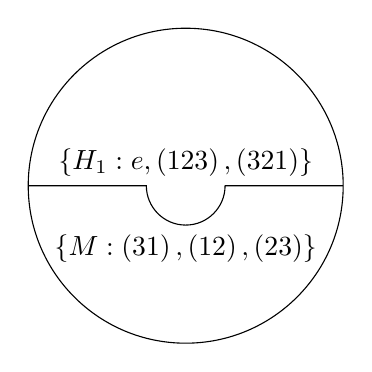
\begin{tikzpicture}
    \draw (0,0) circle [radius=2];
    \draw (2,0) -- (0.5,0) arc [radius=0.5, start angle = 0, end angle = -180] -- (-2,0);
    \node [above] at (0,0) {$\{H_{1}: e, \left(123\right),\left(321\right)\}$};
    \node [below] at (0,-0.5) {$\{M: \left(31\right), \left(12\right), \left(23\right)\}$};
  \end{tikzpicture}
  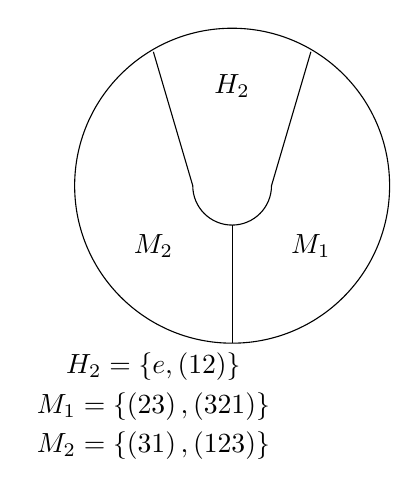
\begin{tikzpicture}
    \draw (0,0) circle [radius=2];
    \draw (1,1.7) -- (0.5,0) arc [radius=0.5, start angle = 0, end angle = -180] -- (-1,1.7);
    \draw (0,-2) -- (0,-0.5);
    \node [above] at (0,1) {$H_{2}$};
    \node [below] at (-1,-0.5) {$M_{2}$};
    \node [below] at (1,-0.5) {$M_{1}$};
    \node [below] at (-1,-2) {$H_{2}= \{e, \left(12\right)\}$};
    \node [below] at (-1,-2.5) {$M_{1}=\{\left(23\right), \left(321\right)\}$};
    \node [below] at (-1,-3) {$M_{2}=\{\left(31\right), \left(123\right)\}$};
  \end{tikzpicture}
  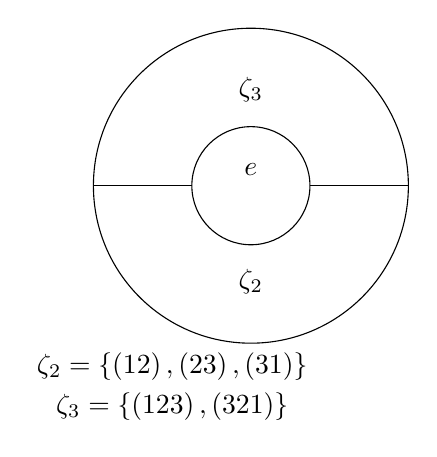
\begin{tikzpicture}
    \draw (0,0) circle [radius=2];
    \draw (0,0) circle [radius=0.75];
    \draw (0.75,0) -- (2,0);
    \draw (-2,0.0) -- (-0.75, 0.0);
    \node [above] at (0,0) {$e$};
    \node [below] at (0,1.5) {$\zeta_{3}$};
    \node [above] at (0,-1.5) {$\zeta_{2}$};
    \node [below] at (-1,-2) {$\zeta_{2}=\{\left(12\right), \left(23\right), \left(31\right)\}$};
    \node [below] at (-1,-2.5) {$\zeta_{3} = \{\left(123\right), \left(321\right)\}$};
  \end{tikzpicture}
  \caption{(a) left cosets of $H_1$ (b) left cosets of $H_2$ (c) classes of $S_3$.}
  \label{fig:1-3}
\end{marginfigure}

The cosets of invariant subgrous are particularly simple and useful.
First, if $H$ is an invariant subgroup, its left cosets are also right cosets\footnote{If $H$ is invariant subgroup $p H p^{-1} = H$, this implies $pH = Hp$.}.
The partitioning of the elements of the full group $G$ into cosets is unique, and a ``factorization'' of $G$ based on this partioning becomes natural.
Let us consider the cosets of an invariant subgroup $H$ as elements of a new group.
The multiplication of two cosets $pH$ and $qH$ is defined as the coset consisting of all products $ph_{i}qh_{j} = \left(pq\right)h_{k}$, where $h_{k} = \left(q^{-1} h_{i} q \right) h_{j} \in H$ provided $h_{i},h_{j} \in H$ and $p,q \in G$.
Since $pH \cdot qH = \left(pq\right) H$, it becomes obvious that (i) $H=eH$ plays the role of the iendtity element; (ii) $p^{-1}H$ is the inverse of $pH$; and (iii) $pH \left(qH \cdot rH \right) = \left(p H \cdot qH \right) \cdot rH = \left(pqr\right) H$.

\textbf{Theorem 1.4} If $H$ is an invarian subgroup of $G$, the set of cosets endowed with the law of multiplication $pH \cdot qH = \left(pq\right)H$ form a group, called the \textit{factor or quotient} group of $G$.
The factor group is denote by $G/H$, it is of order $n_{G}/n_{H}$.

\textrm{Exampel 1}: Consider the inveriant subgroup $H= \{e, a^{2}\}$ of the cyclic group $C_{4}$.
$H$ and coset $M=\{a, a^{3}\}$ form the factor group $C_{4}/H$.
Applying the rule of multiplication of cosets described above, it is straight forward to verify that $HM = M = MH$, $HH = H$, and $MM = H$.
We see that both the subgroup $H$ and the factor group $C_{4}/H$ are of order $2$ and are isomorphic to $C_{2}$.

\textrm{Example 2}: In the case of the permutation group $S_{3}$, $H=\{e, \left(123\right), \left(321\right)\}$ represents an invariant subgroup in Fig.~\ref{fig:1-3} and Tab.~\ref{tab:1-4}.
$G/H$ consists of two elements: $H$ and $M=\{\left(12\right), \left(23\right), \left(31\right)\}$.
We have: $HM= H\cdot \left(ij\right)H= \left(ij\right) H = M = MH$, and $HH= MM = H$.
Therefor, $G/H$ is also isomorphic to the cyclic group of order $2$, $C_{2}$.

\textrm{Example 3}: Consider the discrete translation group $T^{d}=\equiv \Gamma$ and one of its invariant subgroups $\Gamma_{m}$.
The cosets are $\Gamma_{m}$, $T\left(1\right) \Gamma_{m}$, $T\left(2\right) \Gamma_{m}$, \ldots, $T\left(m-1\right) \Gamma_{m}$ and $T\left(m\right) \Gamma_{m} = \Gamma_{m}$.
Hence the factor group $\Gamma/\Gamma_{m}$ is isomorphic to the cyclic group $C_{m}$.
Infinite groups, such as this one, do not behave exactly like finite ones.
For instance, $\Gamma$  and $\Gamma_{m}$ are, in fact, isomorphic to each other even though $\Gamma/\Gamma_{m}$ is non-trival.

\textrm{Example 4}: We state without proof that the translations in $3-$dimensional space form a invariant subgroup of the Euclidean group $E_{3}$; and the factor group is isomrophic to the group of rotations.
This fact forms the basis of important techniques to analyze the Euclidean group and its generalization to $4-$dimensional spacetime---the Poincar\'{e} group.

\section{Homorphisms}
\textbf{Definition 1.11} (homomorphism): A \textit{homomorphism} from a group $G$ to another group $G'$ is a mapping (not necessarily one-to-one) which preserves group multiplication.
In other words, if $g_{i} \in G \to g_{i} \to g_{i}' \in G'$ and $g_{1}g_{2}=g_{3}$, then $g_{1}'g_{2}'=g_{3}'$.

Clearly, isomorphism is a special case of homomorphism.
\begin{figure}
  \centering
    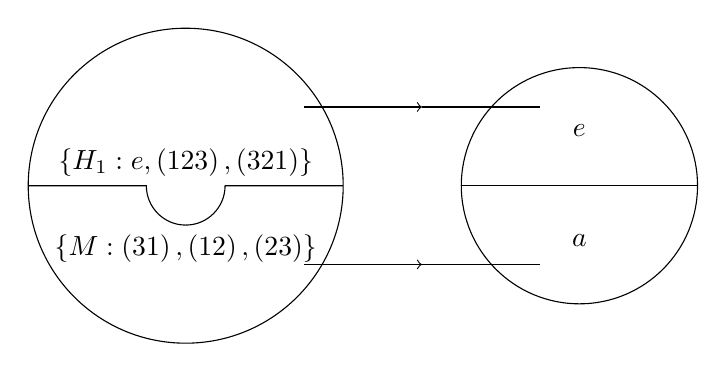
\begin{tikzpicture}
    \draw (0,0) circle [radius=2];
    \draw (2,0) -- (0.5,0) arc [radius=0.5, start angle = 0, end angle = -180] -- (-2,0);
    \node [above] at (0,0) {$\{H_{1}: e, \left(123\right),\left(321\right)\}$};
    \node [below] at (0,-0.5) {$\{M: \left(31\right), \left(12\right), \left(23\right)\}$};
    \draw (5,0) circle [radius=1.5];
    \draw [->] (1.5,1) -- (3,1);
    \draw (3,1) -- (4.5,1);
    \draw [->] (1.5,-1) -- (3,-1);
    \draw (3,-1) -- (4.5,-1);
    \draw (3.5, 0) -- (6.5, 0);
    \node [above] at (5,0.5) {$e$};
    \node [below] at (5,-0.5) {$a$};
  \end{tikzpicture}
  \caption{Homomorphism from $S_3$ to $C_2$.}
  \label{fig:1-4}
\end{figure}

\textrm{Example}:  The mapping from $S_{3}$ to $C_{2}$ depicted in Fig.~\ref{fig:1-4} is a homomorphism.
This follows from the fact that the product of any two element s from $H$ or from $M$ results in an element in H, whereas the product of one element from $H$ with on element from $M$ results in an element in $M$.
This example illustrates the general result that if $G$ has an invariant subgroup $H$, then there exists a natural homomorphism from $G$ to the factor group $G/H: g\in G \to gH \in G/H$.
Group multiplication is preserved b definition.
This result can be turned around to ield the following interesting theorem.

\textbf{Theorem 1.5}: Let $f$ be a homomorphism form $G$ to $G'$.
Denote by $K$ the set of all elements of $G$ whare are mapped to the identity element of $G'$, i.e. $K= \{a \in G; f(a) = e' \in G'\}$.
Then $K$ forms an invariant subgroup of $G$.
Furthermore, the factor group $G/K$ is isomorphic to $G'$.

\section{Direct Products}
Many physically useful symmetry groups are direct products of simpler groups.
When this is the case, it suffices to know the structure and the representations of the smaller groups.

\textbf{Definition 1.12} (Direct Product Group): Let $H_{1}$ and $H_{2}$ be subgroups of a group $G$ with the following properties: (i) every element of $H_{1}$ commutes with any element of $H_{2}$, i.e. $h_{1}h_{2} = h_{2} h_{1}$ for $\forall h_{1} \in H_{1}$ and $\forall h_{2}\in H_{2}$; and (ii) every element $g$ for $G$ can be written uniquely as $g=h_{1}h_{2}$ where $h_{1}\in H_{1}$ and $h_{2}\in H_{2}$.
In this case, $G$ is said to be the direct product of $H_{1}$ and $H_{2}$; symbolically, $G= H_{1}\otimes H_{2}$.

\textrm{Example 1}: Consider the group $C_{6}$ with elements $\{e = a^{6}, a, a^{2}, a^{3}, a^{4}, a^{5}\}$, and the subgroups $H_{1} = \{e, a^{3}\}$ and $H_{2} = \{e, a^{2}, a^{4}\}$.
Cirterion (i)is trivally satisfied because the group is abelian, and (ii) can be verified by $e=ee$, $a = a^{3} a^{4}$ and so on.
Since $H_{1}$ and $H_{2}$ are isomorpism to $C_{2}$ and $C_{3}$, i.e. $H_{1} \simeq C_{2}$ and $H_{2} \simeq C_{3}$, we have $C_{6} \simeq C_{2} \otimes C_{3}$.

If $G= H_{1}\otimes H_{2}$, then both $H_{1}$ and $H_{2}$ must be invariant subgroups of $G$.
\footnote{If $g=h_{1}h_{2}\in G$, and $h_{1}, a \in H_{1}$, $h_{2}\in H_{2}$. Then $g a g^{-1} = h_{1}h_{2} a h_{2}^{-1} h_{1}^{-1} = h_{1} a h_{1}^{-1} \in H_{1}$ for all $g$ and $a$.}
Now, we can form the quotient group $G/H_{2}$ and prove that, $G/H_{2} \simeq H_{1}$.
However, the converse to the above is not true!
Let $H$ be an invariant subgroup of $G$ and $H'= G/H$.
It does not follow that $G = H \otimes H'$.


%%% Local Variables:
%%% mode: latex
%%% TeX-master: "main"
%%% End:
